% 第4章第1节：集合函数（集合函数的定义；子集与二值向量；边际增益）。

\section{集合函数}
\label{sec:graph-set-function-basics}

给每个元素赋一个数，只需要一张长度为元素个数的表；给每个子集赋一个数，则要考虑元素之间怎样相互影响。本节先用传感器覆盖说明为什么需要以子集为自变量的函数，再把子集写成二值向量，最后定义新增一个元素带来的评价变化。这三样东西是后面判断函数性质、设计选择方法时共同使用的记号。

\subsection{集合函数的定义}
\label{sec:graph-setfn-definition}

\paragraph{传感器覆盖实例}
图~\ref{fig:graph-setfn-sensor-coverage}是一块由上下两行、左右八列组成的区域，共$16$个格子。有四个候选传感器：$a$覆盖第$2$至$6$列的$10$个格子，$b$覆盖第$1$至$4$列的$8$个格子，$c$覆盖第$5$至$8$列的$8$个格子，$d$只覆盖左上角的$1$个格子。选定一组传感器后，我们关心这组传感器合起来覆盖了多少个不同的格子。记传感器$v$覆盖的格子集合为$C_v$，选定的传感器集合为$S$，覆盖量就是
\[
  F(S)=\Bigl|\bigcup_{v\in S}C_v\Bigr|.
\]
单独看，$F(\{a\})=10$，$F(\{b\})=8$；两者一起时，第$2$至$4$列被重复覆盖，$F(\{a,b\})=12$，而不是$10+8=18$。整组的价值不能由各成员的价值相加得到，因此评价必须直接以“哪些传感器被选中”为输入。本章后面几节都用这个实例做算例。

\begin{figure}[!htb]
  \centering
  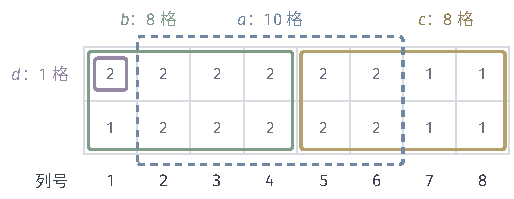
\includegraphics[width=87.027mm]{figures/01-basic-mathematics/04-graphs/tikz/c4-sensor-coverage/figure.pdf}
  \caption{贯穿本章的传感器覆盖实例。区域由$2\times 8$个格子组成；绿色框为$b$（第$1$至$4$列），黄色框为$c$（第$5$至$8$列），蓝色虚线框为$a$（第$2$至$6$列），紫色小框为$d$（左上角一格）。格内数字是覆盖该格的传感器个数，数字$2$所在的格子都被重复覆盖，因而各传感器覆盖格数之和大于它们合起来覆盖的格数。}
  \label{fig:graph-setfn-sensor-coverage}
\end{figure}

覆盖量的输入是一个子集，输出是一个实数。把这种对应一般化，就得到下面的定义。

\begin{definition}[集合函数]
\label{def:graph-setfn-set-function}
设$V$是有限集合，称为\term{底集}（ground set）。把$V$的每个子集对应到一个实数的映射
\[
  F:\mathcal P(V)\to\mathbb R
\]
称为$V$上的\term{集合函数}（set function），其中$\mathcal P(V)$是$V$的幂集。
\end{definition}

定义要求$F$在每个子集上都有值，包括空集。空集表示“什么都不选”，它的值是比较其他选择的起点：覆盖量取$F(\varnothing)=0$，一个带固定开销的评价则可能取非零值。底集中的元素可以是传感器、特征、顶点或边；集合函数本身并不要求底集带有图结构。

\paragraph{三个例子}
同一个子集可以按不同目的评价。以传感器实例为例，给四个传感器分别指定安装成本$4,3,4,1$（依次对应$a,b,c,d$），总成本
\[
  c(S)=\sum_{v\in S}c_v
\]
是一个集合函数，例如$c(\{a,b\})=7$；覆盖量$F$是另一个集合函数，$F(\{a,b\})=12$。第三个例子来自图。设$\mathcal G=(V,E)$是无向图，每条边$\{i,j\}$带非负权$w_{i,j}$。顶点子集$S$把顶点分成$S$与$V\setminus S$两侧，这正是第~\ref{sec:graph-minimum-spanning-tree}节所说的割；两端分居两侧的边的权之和
\[
  \operatorname{cut}(S)=\sum_{\{i,j\}\in E:\ |\{i,j\}\cap S|=1}w_{i,j}
\]
称为$S$的割权。这里的底集是顶点集，$\operatorname{cut}$以顶点子集为自变量。三个例子分别累计单项成本、合并覆盖范围和统计跨越两侧的边，元素之间的相互影响各不相同，下一节将据此区分它们的性质。

\paragraph{取值表与求值规则}
由式~\eqref{eq:comb-power-set-count}，$n$元底集有$2^n$个子集，所以一个集合函数的完整取值表有$2^n$项。传感器实例只有$16$项，可以全部写出；底集有$50$个元素时，取值表已超过$10^{15}$项，无法存储。实际问题中的集合函数通常由一条规则给出：给定$S$，按规则算出$F(S)$。覆盖量的规则是求并集再计数，割权的规则是扫描全部边。这样的一次计算称为一次\emph{求值}，它的代价取决于具体表示：覆盖量的一次求值要处理$S$中各传感器的覆盖范围，割权的一次求值要检查每条边。后面分析算法时，我们把求值次数和每次求值的代价分开计算，不把求值默认视为免费。

\subsection{子集与二值向量}
\label{sec:graph-setfn-binary-vectors}

给底集的元素固定编号$V=\{1,\ldots,n\}$。第~\ref{sec:comb-ordered-unordered}节已经说明，子集$S$与零一记录一一对应。把这条记录写成向量$\bm x=(x_1,\ldots,x_n)\in\{0,1\}^n$，其中
\[
  x_i=\mathbb I\{i\in S\},
\]
称$\bm x$为$S$的\term{指示向量}（indicator vector）。反过来，由$\bm x$恢复子集只需收集取值为$1$的坐标：$S=\{i:x_i=1\}$。

集合运算在指示向量上逐坐标进行。设$S,T$的指示向量为$\bm x,\bm y$，则元素个数是坐标之和，$|S|=\sum_ix_i$；并集的第$i$个坐标是$\max\{x_i,y_i\}$，交集的第$i$个坐标是$\min\{x_i,y_i\}=x_iy_i$，补集的第$i$个坐标是$1-x_i$。包含关系$S\subseteq T$对应逐坐标的$x_i\leq y_i$。

于是集合函数也可以写成二值向量的函数：令$f(\bm x)=F(\{i:x_i=1\})$，$f$与$F$只是同一组数值的两种索引方式。图~\ref{fig:graph-setfn-subset-binary-cube}以三元底集为例画出这一对应：八个子集恰好是立方体的八个顶点，立方体的每条边连接只差一个元素的两个子集，也就是只差一个坐标的两个向量。

\begin{figure}[!htb]
  \centering
  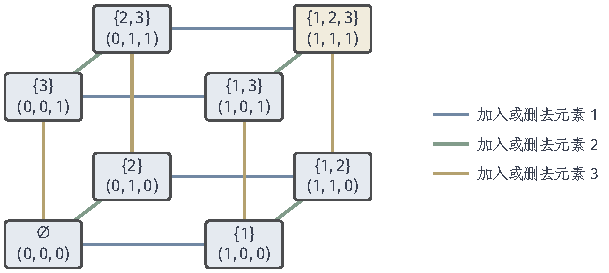
\includegraphics[width=103.209mm]{figures/01-basic-mathematics/04-graphs/tikz/c4-subset-binary-cube/figure.pdf}
  \caption{三元底集$V=\{1,2,3\}$的八个子集与指示向量$(x_1,x_2,x_3)$排成立方体的顶点。每个框上行是子集，下行是对应的向量；边的颜色表示沿这条边加入或删去哪个元素，也就是改变哪个坐标。沿任一条边向上走一步，就是在当前子集中加入一个元素。}
  \label{fig:graph-setfn-subset-binary-cube}
\end{figure}

这一改写只换了表示方式，并没有带来额外结构。写成$f(\bm x)$之后，$f$不一定是各坐标的函数之和，也不一定能分解成只读取少数坐标的局部项；在$\{0,1\}^n$上谈连续性或求导也没有意义。第~\ref{sec:graph-pairwise-binary-cut}节和第~\ref{chap:graph-dynamic-programming}章讨论的，正是函数确实具有某种局部分解时可以怎样利用它。

\subsection{边际增益}
\label{sec:graph-setfn-marginal-gain}

选择子集时，最直接的问题是：在已经选好的集合上再加一个元素，评价会改变多少。

\begin{definition}[边际增益]
\label{def:graph-setfn-marginal-gain}
设$F$是$V$上的集合函数，$S\subseteq V$，$v\in V\setminus S$。称
\[
  \Delta(v\mid S)=F(S\cup\{v\})-F(S)
\]
为元素$v$相对于集合$S$的\term{边际增益}（marginal gain）。
\end{definition}

边际增益同时依赖新元素和已选集合。图~\ref{fig:graph-setfn-marginal-gain-overlap}比较同一个传感器$c$在两种情况下的增益：从空集加入时，$c$的$8$个格子都是新覆盖的，$\Delta(c\mid\varnothing)=8$；已经选了$a$之后，$c$的第$5$、$6$列已被$a$覆盖，只有第$7$、$8$列的$4$个格子是新的，$\Delta(c\mid\{a\})=4$。所以谈论一个元素“值多少”时，必须说明是相对于哪个已选集合。

\begin{figure}[!htb]
  \centering
  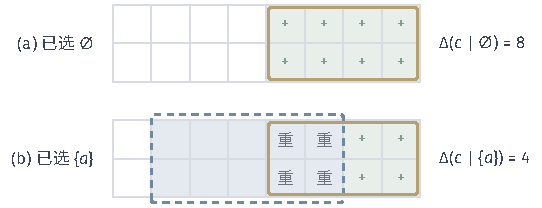
\includegraphics[width=91.74mm]{figures/01-basic-mathematics/04-graphs/tikz/c4-marginal-gain-overlap/figure.pdf}
  \caption{同一传感器$c$（黄色框）的边际增益随已选集合变化。(a) 已选集合为空，$c$覆盖的$8$个格子（绿色，标“$+$”）全部是新覆盖；(b) 已选$\{a\}$（蓝色底与蓝色虚线框），$c$与$a$重叠的第$5$、$6$列（标“重”）不再计数，只有第$7$、$8$列的$4$个格子是新覆盖。}
  \label{fig:graph-setfn-marginal-gain-overlap}
\end{figure}

\paragraph{逐个加入的累计}
把一个集合的元素逐个加入，函数的总变化就是一串边际增益之和。设$A\subseteq B\subseteq V$，把$B\setminus A$中的元素按任意次序排成$v_1,\ldots,v_r$，记$A_0=A$，$A_k=A\cup\{v_1,\ldots,v_k\}$。于是$A_r=B$，并且
\begin{equation}
  F(B)-F(A)=\sum_{k=1}^{r}\bigl(F(A_k)-F(A_{k-1})\bigr)=\sum_{k=1}^{r}\Delta(v_k\mid A_{k-1}).
  \label{eq:graph-setfn-telescoping}
\end{equation}
第一个等号是裂项求和（式~\eqref{eq:prelim-telescoping-sum}）：中间的$F(A_1),\ldots,F(A_{r-1})$各出现一次正号、一次负号而抵消。第二个等号是因为$A_k=A_{k-1}\cup\{v_k\}$且$v_k\notin A_{k-1}$。

在传感器实例中取$A=\varnothing$、$B=\{a,b,c\}$。按$a,c,b$的次序加入，三个增益依次是$10,4,2$；按$b,c,a$的次序加入，三个增益依次是$8,8,0$。两种次序的总和都是$F(\{a,b,c\})=16$，但每一步的增益随次序改变。式~\eqref{eq:graph-setfn-telescoping}是下一节判别性质和第~\ref{sec:graph-cardinality-selection}节分析贪心算法的共同工具。

边际增益只描述一步的变化。在空集上，$a$的增益$10$是四个传感器中最大的，但只能选两个传感器时，最好的组合是$\{b,c\}$，它覆盖全部$16$个格子，并不包含$a$。单步增益大，不保证这一步属于某个全局最优子集；这一点将在第~\ref{sec:graph-cardinality-selection}节具体比较。
